% The RDM truncation as a procedure, for the introduction of the truncation appendix.
% Three steps, left to right, one operation each:
%   (a) the chain in mixed canonical form, every physical leg open;
%   (b) the indices on either side of the centre grouped into composite indices, drawn as thick
%       lines, so the cut is a matrix and its decomposition carries an internal index chi;
%   (c) the same picture after truncation, the internal index reduced to chi'.
% (b) and (c) deliberately show the same object, so the truncation reads as one index shrinking.
% From (b) onward the picture stays in the matrix representation: the composite legs remain thick
% and no open physical leg reappears.
% Colours, tensor shapes and line weights follow imgs/truncation.tex.
%
% Standalone: compiles to imgs/rdm_pipeline.pdf.
% Inline:     with \usepackage{standalone}, % The RDM truncation as a procedure, for the introduction of the truncation appendix.
% Three steps, left to right, one operation each:
%   (a) the chain in mixed canonical form, every physical leg open;
%   (b) the indices on either side of the centre grouped into composite indices, drawn as thick
%       lines, so the cut is a matrix and its decomposition carries an internal index chi;
%   (c) the same picture after truncation, the internal index reduced to chi'.
% (b) and (c) deliberately show the same object, so the truncation reads as one index shrinking.
% From (b) onward the picture stays in the matrix representation: the composite legs remain thick
% and no open physical leg reappears.
% Colours, tensor shapes and line weights follow imgs/truncation.tex.
%
% Standalone: compiles to imgs/rdm_pipeline.pdf.
% Inline:     with \usepackage{standalone}, % The RDM truncation as a procedure, for the introduction of the truncation appendix.
% Three steps, left to right, one operation each:
%   (a) the chain in mixed canonical form, every physical leg open;
%   (b) the indices on either side of the centre grouped into composite indices, drawn as thick
%       lines, so the cut is a matrix and its decomposition carries an internal index chi;
%   (c) the same picture after truncation, the internal index reduced to chi'.
% (b) and (c) deliberately show the same object, so the truncation reads as one index shrinking.
% From (b) onward the picture stays in the matrix representation: the composite legs remain thick
% and no open physical leg reappears.
% Colours, tensor shapes and line weights follow imgs/truncation.tex.
%
% Standalone: compiles to imgs/rdm_pipeline.pdf.
% Inline:     with \usepackage{standalone}, % The RDM truncation as a procedure, for the introduction of the truncation appendix.
% Three steps, left to right, one operation each:
%   (a) the chain in mixed canonical form, every physical leg open;
%   (b) the indices on either side of the centre grouped into composite indices, drawn as thick
%       lines, so the cut is a matrix and its decomposition carries an internal index chi;
%   (c) the same picture after truncation, the internal index reduced to chi'.
% (b) and (c) deliberately show the same object, so the truncation reads as one index shrinking.
% From (b) onward the picture stays in the matrix representation: the composite legs remain thick
% and no open physical leg reappears.
% Colours, tensor shapes and line weights follow imgs/truncation.tex.
%
% Standalone: compiles to imgs/rdm_pipeline.pdf.
% Inline:     with \usepackage{standalone}, \input{imgs/rdm_pipeline}.
\documentclass[tikz,border=3pt]{standalone}
\usepackage{amsmath,amssymb,braket,graphicx}
\usetikzlibrary{arrows.meta,shapes.geometric}

\definecolor{ketc}{RGB}{150,215,240}
\definecolor{brac}{RGB}{60,130,175}
\definecolor{ctrk}{RGB}{250,200,150}
\definecolor{ctrb}{RGB}{225,140,60}

\newcommand{\DX}{0.90}    % spacing between neighbouring tensors
\newcommand{\ST}{0.44}    % length of an open physical leg

\newcommand{\Dhh}{0.21}   % half-height of a tensor
\newcommand{\Dbb}{0.21}   % straight body, so the D is as wide as it is tall

% D-shaped tensors centred at (#1,#2), filled #3; \dR has its flat edge left, \dL right
\newcommand{\dR}[3]{%
  \filldraw[fill=#3, draw=black, line width=1.1pt]
    ({#1-(\Dbb+\Dhh)/2},{#2-\Dhh}) -- ({#1+(\Dbb-\Dhh)/2},{#2-\Dhh})
    arc[start angle=-90, end angle=90, radius=\Dhh]
    -- ({#1-(\Dbb+\Dhh)/2},{#2+\Dhh}) -- cycle;}
\newcommand{\dL}[3]{%
  \filldraw[fill=#3, draw=black, line width=1.1pt]
    ({#1+(\Dbb+\Dhh)/2},{#2-\Dhh}) -- ({#1-(\Dbb-\Dhh)/2},{#2-\Dhh})
    arc[start angle=-90, end angle=-270, radius=\Dhh]
    -- ({#1+(\Dbb+\Dhh)/2},{#2+\Dhh}) -- cycle;}

\begin{document}
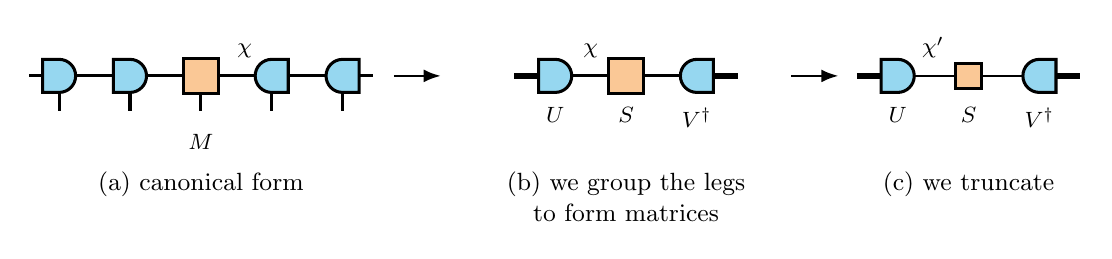
\begin{tikzpicture}[
    bond/.style={draw=black, line width=1.1pt},
    fat/.style={draw=black, line width=2.4pt},
    Sq/.style={rectangle, draw=black, line width=1.1pt, minimum size=4.4mm, inner sep=0pt},
    Sqcut/.style={rectangle, draw=black, line width=1.1pt, minimum size=3.2mm, inner sep=0pt},
    cut bond/.style={draw=black, line width=0.7pt},
    flow/.style={-{Latex[length=2.2mm]}, line width=1.0pt},
    tag/.style={font=\small, align=center},
    idx/.style={font=\footnotesize},
  ]

  % --- (a) mixed canonical form, orthogonality centre on the cut bond
  \begin{scope}
    \draw[bond] (-0.38,0) -- ({4*\DX+0.38},0);
    \foreach \i in {0,1,2,3,4} { \draw[bond] (\i*\DX,0) -- (\i*\DX,-\ST); }
    \dR{0}{0}{ketc}
    \dR{\DX}{0}{ketc}
    \node[Sq, fill=ctrk] at ({2*\DX},0) {};
    \dL{3*\DX}{0}{ketc}
    \dL{4*\DX}{0}{ketc}
    \node[idx, anchor=south] at ({2.62*\DX},0.10) {$\chi$};
    \node[idx, anchor=north] at ({2*\DX},-0.62) {$M$};
    \node[tag, anchor=north] at ({2*\DX},-1.10) {(a) canonical form};
  \end{scope}

  \draw[flow] (4.25,0) -- (4.85,0);

  % --- (b) the cut as a matrix: composite legs thick, decomposition at internal index chi
  \begin{scope}[xshift=6.30cm]
    \draw[fat]  (-0.52,0) -- (-0.16,0);
    \draw[bond] (-0.16,0) -- ({2*\DX+0.16},0);
    \draw[fat]  ({2*\DX+0.16},0) -- ({2*\DX+0.52},0);
    \dR{0}{0}{ketc}
    \node[Sq, fill=ctrk] at (\DX,0) {};
    \dL{2*\DX}{0}{ketc}
    \node[idx, anchor=south] at ({0.5*\DX},0.10) {$\chi$};
    \node[idx, anchor=north] at (0,-0.28) {$U$};
    \node[idx, anchor=north] at (\DX,-0.28) {$S$};
    \node[idx, anchor=north] at ({2*\DX},-0.28) {$V^{\dagger}$};
    \node[tag, anchor=north] at (\DX,-1.10) {(b) we group the legs\\to form matrices};
  \end{scope}

  \draw[flow] (9.30,0) -- (9.90,0);

  % --- (c) the same object after truncation: internal index chi', drawn thinner
  \begin{scope}[xshift=10.65cm]
    \draw[fat]      (-0.52,0) -- (-0.16,0);
    \draw[cut bond] (-0.16,0) -- ({2*\DX+0.16},0);
    \draw[fat]      ({2*\DX+0.16},0) -- ({2*\DX+0.52},0);
    \dR{0}{0}{ketc}
    \node[Sqcut, fill=ctrk] at (\DX,0) {};
    \dL{2*\DX}{0}{ketc}
    \node[idx, anchor=south] at ({0.5*\DX},0.10) {$\chi'$};
    \node[idx, anchor=north] at (0,-0.28) {$U$};
    \node[idx, anchor=north] at (\DX,-0.28) {$S$};
    \node[idx, anchor=north] at ({2*\DX},-0.28) {$V^{\dagger}$};
    \node[tag, anchor=north] at (\DX,-1.10) {(c) we truncate};
  \end{scope}

\end{tikzpicture}
\end{document}
.
\documentclass[tikz,border=3pt]{standalone}
\usepackage{amsmath,amssymb,braket,graphicx}
\usetikzlibrary{arrows.meta,shapes.geometric}

\definecolor{ketc}{RGB}{150,215,240}
\definecolor{brac}{RGB}{60,130,175}
\definecolor{ctrk}{RGB}{250,200,150}
\definecolor{ctrb}{RGB}{225,140,60}

\newcommand{\DX}{0.90}    % spacing between neighbouring tensors
\newcommand{\ST}{0.44}    % length of an open physical leg

\newcommand{\Dhh}{0.21}   % half-height of a tensor
\newcommand{\Dbb}{0.21}   % straight body, so the D is as wide as it is tall

% D-shaped tensors centred at (#1,#2), filled #3; \dR has its flat edge left, \dL right
\newcommand{\dR}[3]{%
  \filldraw[fill=#3, draw=black, line width=1.1pt]
    ({#1-(\Dbb+\Dhh)/2},{#2-\Dhh}) -- ({#1+(\Dbb-\Dhh)/2},{#2-\Dhh})
    arc[start angle=-90, end angle=90, radius=\Dhh]
    -- ({#1-(\Dbb+\Dhh)/2},{#2+\Dhh}) -- cycle;}
\newcommand{\dL}[3]{%
  \filldraw[fill=#3, draw=black, line width=1.1pt]
    ({#1+(\Dbb+\Dhh)/2},{#2-\Dhh}) -- ({#1-(\Dbb-\Dhh)/2},{#2-\Dhh})
    arc[start angle=-90, end angle=-270, radius=\Dhh]
    -- ({#1+(\Dbb+\Dhh)/2},{#2+\Dhh}) -- cycle;}

\begin{document}
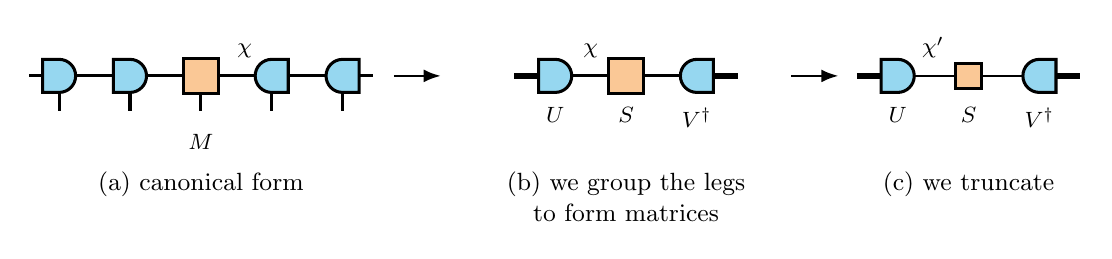
\begin{tikzpicture}[
    bond/.style={draw=black, line width=1.1pt},
    fat/.style={draw=black, line width=2.4pt},
    Sq/.style={rectangle, draw=black, line width=1.1pt, minimum size=4.4mm, inner sep=0pt},
    Sqcut/.style={rectangle, draw=black, line width=1.1pt, minimum size=3.2mm, inner sep=0pt},
    cut bond/.style={draw=black, line width=0.7pt},
    flow/.style={-{Latex[length=2.2mm]}, line width=1.0pt},
    tag/.style={font=\small, align=center},
    idx/.style={font=\footnotesize},
  ]

  % --- (a) mixed canonical form, orthogonality centre on the cut bond
  \begin{scope}
    \draw[bond] (-0.38,0) -- ({4*\DX+0.38},0);
    \foreach \i in {0,1,2,3,4} { \draw[bond] (\i*\DX,0) -- (\i*\DX,-\ST); }
    \dR{0}{0}{ketc}
    \dR{\DX}{0}{ketc}
    \node[Sq, fill=ctrk] at ({2*\DX},0) {};
    \dL{3*\DX}{0}{ketc}
    \dL{4*\DX}{0}{ketc}
    \node[idx, anchor=south] at ({2.62*\DX},0.10) {$\chi$};
    \node[idx, anchor=north] at ({2*\DX},-0.62) {$M$};
    \node[tag, anchor=north] at ({2*\DX},-1.10) {(a) canonical form};
  \end{scope}

  \draw[flow] (4.25,0) -- (4.85,0);

  % --- (b) the cut as a matrix: composite legs thick, decomposition at internal index chi
  \begin{scope}[xshift=6.30cm]
    \draw[fat]  (-0.52,0) -- (-0.16,0);
    \draw[bond] (-0.16,0) -- ({2*\DX+0.16},0);
    \draw[fat]  ({2*\DX+0.16},0) -- ({2*\DX+0.52},0);
    \dR{0}{0}{ketc}
    \node[Sq, fill=ctrk] at (\DX,0) {};
    \dL{2*\DX}{0}{ketc}
    \node[idx, anchor=south] at ({0.5*\DX},0.10) {$\chi$};
    \node[idx, anchor=north] at (0,-0.28) {$U$};
    \node[idx, anchor=north] at (\DX,-0.28) {$S$};
    \node[idx, anchor=north] at ({2*\DX},-0.28) {$V^{\dagger}$};
    \node[tag, anchor=north] at (\DX,-1.10) {(b) we group the legs\\to form matrices};
  \end{scope}

  \draw[flow] (9.30,0) -- (9.90,0);

  % --- (c) the same object after truncation: internal index chi', drawn thinner
  \begin{scope}[xshift=10.65cm]
    \draw[fat]      (-0.52,0) -- (-0.16,0);
    \draw[cut bond] (-0.16,0) -- ({2*\DX+0.16},0);
    \draw[fat]      ({2*\DX+0.16},0) -- ({2*\DX+0.52},0);
    \dR{0}{0}{ketc}
    \node[Sqcut, fill=ctrk] at (\DX,0) {};
    \dL{2*\DX}{0}{ketc}
    \node[idx, anchor=south] at ({0.5*\DX},0.10) {$\chi'$};
    \node[idx, anchor=north] at (0,-0.28) {$U$};
    \node[idx, anchor=north] at (\DX,-0.28) {$S$};
    \node[idx, anchor=north] at ({2*\DX},-0.28) {$V^{\dagger}$};
    \node[tag, anchor=north] at (\DX,-1.10) {(c) we truncate};
  \end{scope}

\end{tikzpicture}
\end{document}
.
\documentclass[tikz,border=3pt]{standalone}
\usepackage{amsmath,amssymb,braket,graphicx}
\usetikzlibrary{arrows.meta,shapes.geometric}

\definecolor{ketc}{RGB}{150,215,240}
\definecolor{brac}{RGB}{60,130,175}
\definecolor{ctrk}{RGB}{250,200,150}
\definecolor{ctrb}{RGB}{225,140,60}

\newcommand{\DX}{0.90}    % spacing between neighbouring tensors
\newcommand{\ST}{0.44}    % length of an open physical leg

\newcommand{\Dhh}{0.21}   % half-height of a tensor
\newcommand{\Dbb}{0.21}   % straight body, so the D is as wide as it is tall

% D-shaped tensors centred at (#1,#2), filled #3; \dR has its flat edge left, \dL right
\newcommand{\dR}[3]{%
  \filldraw[fill=#3, draw=black, line width=1.1pt]
    ({#1-(\Dbb+\Dhh)/2},{#2-\Dhh}) -- ({#1+(\Dbb-\Dhh)/2},{#2-\Dhh})
    arc[start angle=-90, end angle=90, radius=\Dhh]
    -- ({#1-(\Dbb+\Dhh)/2},{#2+\Dhh}) -- cycle;}
\newcommand{\dL}[3]{%
  \filldraw[fill=#3, draw=black, line width=1.1pt]
    ({#1+(\Dbb+\Dhh)/2},{#2-\Dhh}) -- ({#1-(\Dbb-\Dhh)/2},{#2-\Dhh})
    arc[start angle=-90, end angle=-270, radius=\Dhh]
    -- ({#1+(\Dbb+\Dhh)/2},{#2+\Dhh}) -- cycle;}

\begin{document}
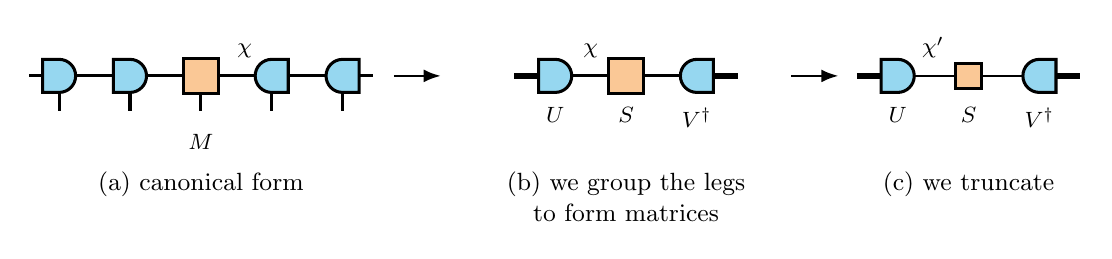
\begin{tikzpicture}[
    bond/.style={draw=black, line width=1.1pt},
    fat/.style={draw=black, line width=2.4pt},
    Sq/.style={rectangle, draw=black, line width=1.1pt, minimum size=4.4mm, inner sep=0pt},
    Sqcut/.style={rectangle, draw=black, line width=1.1pt, minimum size=3.2mm, inner sep=0pt},
    cut bond/.style={draw=black, line width=0.7pt},
    flow/.style={-{Latex[length=2.2mm]}, line width=1.0pt},
    tag/.style={font=\small, align=center},
    idx/.style={font=\footnotesize},
  ]

  % --- (a) mixed canonical form, orthogonality centre on the cut bond
  \begin{scope}
    \draw[bond] (-0.38,0) -- ({4*\DX+0.38},0);
    \foreach \i in {0,1,2,3,4} { \draw[bond] (\i*\DX,0) -- (\i*\DX,-\ST); }
    \dR{0}{0}{ketc}
    \dR{\DX}{0}{ketc}
    \node[Sq, fill=ctrk] at ({2*\DX},0) {};
    \dL{3*\DX}{0}{ketc}
    \dL{4*\DX}{0}{ketc}
    \node[idx, anchor=south] at ({2.62*\DX},0.10) {$\chi$};
    \node[idx, anchor=north] at ({2*\DX},-0.62) {$M$};
    \node[tag, anchor=north] at ({2*\DX},-1.10) {(a) canonical form};
  \end{scope}

  \draw[flow] (4.25,0) -- (4.85,0);

  % --- (b) the cut as a matrix: composite legs thick, decomposition at internal index chi
  \begin{scope}[xshift=6.30cm]
    \draw[fat]  (-0.52,0) -- (-0.16,0);
    \draw[bond] (-0.16,0) -- ({2*\DX+0.16},0);
    \draw[fat]  ({2*\DX+0.16},0) -- ({2*\DX+0.52},0);
    \dR{0}{0}{ketc}
    \node[Sq, fill=ctrk] at (\DX,0) {};
    \dL{2*\DX}{0}{ketc}
    \node[idx, anchor=south] at ({0.5*\DX},0.10) {$\chi$};
    \node[idx, anchor=north] at (0,-0.28) {$U$};
    \node[idx, anchor=north] at (\DX,-0.28) {$S$};
    \node[idx, anchor=north] at ({2*\DX},-0.28) {$V^{\dagger}$};
    \node[tag, anchor=north] at (\DX,-1.10) {(b) we group the legs\\to form matrices};
  \end{scope}

  \draw[flow] (9.30,0) -- (9.90,0);

  % --- (c) the same object after truncation: internal index chi', drawn thinner
  \begin{scope}[xshift=10.65cm]
    \draw[fat]      (-0.52,0) -- (-0.16,0);
    \draw[cut bond] (-0.16,0) -- ({2*\DX+0.16},0);
    \draw[fat]      ({2*\DX+0.16},0) -- ({2*\DX+0.52},0);
    \dR{0}{0}{ketc}
    \node[Sqcut, fill=ctrk] at (\DX,0) {};
    \dL{2*\DX}{0}{ketc}
    \node[idx, anchor=south] at ({0.5*\DX},0.10) {$\chi'$};
    \node[idx, anchor=north] at (0,-0.28) {$U$};
    \node[idx, anchor=north] at (\DX,-0.28) {$S$};
    \node[idx, anchor=north] at ({2*\DX},-0.28) {$V^{\dagger}$};
    \node[tag, anchor=north] at (\DX,-1.10) {(c) we truncate};
  \end{scope}

\end{tikzpicture}
\end{document}
.
\documentclass[tikz,border=3pt]{standalone}
\usepackage{amsmath,amssymb,braket,graphicx}
\usetikzlibrary{arrows.meta,shapes.geometric}

\definecolor{ketc}{RGB}{150,215,240}
\definecolor{brac}{RGB}{60,130,175}
\definecolor{ctrk}{RGB}{250,200,150}
\definecolor{ctrb}{RGB}{225,140,60}

\newcommand{\DX}{0.90}    % spacing between neighbouring tensors
\newcommand{\ST}{0.44}    % length of an open physical leg

\newcommand{\Dhh}{0.21}   % half-height of a tensor
\newcommand{\Dbb}{0.21}   % straight body, so the D is as wide as it is tall

% D-shaped tensors centred at (#1,#2), filled #3; \dR has its flat edge left, \dL right
\newcommand{\dR}[3]{%
  \filldraw[fill=#3, draw=black, line width=1.1pt]
    ({#1-(\Dbb+\Dhh)/2},{#2-\Dhh}) -- ({#1+(\Dbb-\Dhh)/2},{#2-\Dhh})
    arc[start angle=-90, end angle=90, radius=\Dhh]
    -- ({#1-(\Dbb+\Dhh)/2},{#2+\Dhh}) -- cycle;}
\newcommand{\dL}[3]{%
  \filldraw[fill=#3, draw=black, line width=1.1pt]
    ({#1+(\Dbb+\Dhh)/2},{#2-\Dhh}) -- ({#1-(\Dbb-\Dhh)/2},{#2-\Dhh})
    arc[start angle=-90, end angle=-270, radius=\Dhh]
    -- ({#1+(\Dbb+\Dhh)/2},{#2+\Dhh}) -- cycle;}

\begin{document}
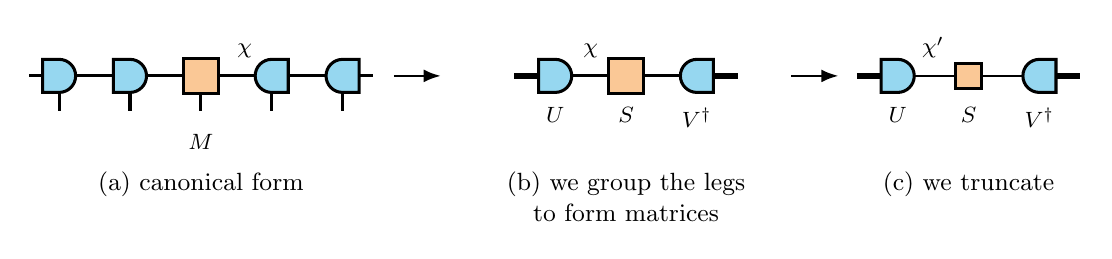
\begin{tikzpicture}[
    bond/.style={draw=black, line width=1.1pt},
    fat/.style={draw=black, line width=2.4pt},
    Sq/.style={rectangle, draw=black, line width=1.1pt, minimum size=4.4mm, inner sep=0pt},
    Sqcut/.style={rectangle, draw=black, line width=1.1pt, minimum size=3.2mm, inner sep=0pt},
    cut bond/.style={draw=black, line width=0.7pt},
    flow/.style={-{Latex[length=2.2mm]}, line width=1.0pt},
    tag/.style={font=\small, align=center},
    idx/.style={font=\footnotesize},
  ]

  % --- (a) mixed canonical form, orthogonality centre on the cut bond
  \begin{scope}
    \draw[bond] (-0.38,0) -- ({4*\DX+0.38},0);
    \foreach \i in {0,1,2,3,4} { \draw[bond] (\i*\DX,0) -- (\i*\DX,-\ST); }
    \dR{0}{0}{ketc}
    \dR{\DX}{0}{ketc}
    \node[Sq, fill=ctrk] at ({2*\DX},0) {};
    \dL{3*\DX}{0}{ketc}
    \dL{4*\DX}{0}{ketc}
    \node[idx, anchor=south] at ({2.62*\DX},0.10) {$\chi$};
    \node[idx, anchor=north] at ({2*\DX},-0.62) {$M$};
    \node[tag, anchor=north] at ({2*\DX},-1.10) {(a) canonical form};
  \end{scope}

  \draw[flow] (4.25,0) -- (4.85,0);

  % --- (b) the cut as a matrix: composite legs thick, decomposition at internal index chi
  \begin{scope}[xshift=6.30cm]
    \draw[fat]  (-0.52,0) -- (-0.16,0);
    \draw[bond] (-0.16,0) -- ({2*\DX+0.16},0);
    \draw[fat]  ({2*\DX+0.16},0) -- ({2*\DX+0.52},0);
    \dR{0}{0}{ketc}
    \node[Sq, fill=ctrk] at (\DX,0) {};
    \dL{2*\DX}{0}{ketc}
    \node[idx, anchor=south] at ({0.5*\DX},0.10) {$\chi$};
    \node[idx, anchor=north] at (0,-0.28) {$U$};
    \node[idx, anchor=north] at (\DX,-0.28) {$S$};
    \node[idx, anchor=north] at ({2*\DX},-0.28) {$V^{\dagger}$};
    \node[tag, anchor=north] at (\DX,-1.10) {(b) we group the legs\\to form matrices};
  \end{scope}

  \draw[flow] (9.30,0) -- (9.90,0);

  % --- (c) the same object after truncation: internal index chi', drawn thinner
  \begin{scope}[xshift=10.65cm]
    \draw[fat]      (-0.52,0) -- (-0.16,0);
    \draw[cut bond] (-0.16,0) -- ({2*\DX+0.16},0);
    \draw[fat]      ({2*\DX+0.16},0) -- ({2*\DX+0.52},0);
    \dR{0}{0}{ketc}
    \node[Sqcut, fill=ctrk] at (\DX,0) {};
    \dL{2*\DX}{0}{ketc}
    \node[idx, anchor=south] at ({0.5*\DX},0.10) {$\chi'$};
    \node[idx, anchor=north] at (0,-0.28) {$U$};
    \node[idx, anchor=north] at (\DX,-0.28) {$S$};
    \node[idx, anchor=north] at ({2*\DX},-0.28) {$V^{\dagger}$};
    \node[tag, anchor=north] at (\DX,-1.10) {(c) we truncate};
  \end{scope}

\end{tikzpicture}
\end{document}
